\documentclass[a5paper]{book}
\usepackage{import}
\usepackage[spanish,french]{bilingue}

\begin{document}

\title{Es que somos muy pobres\\
	\normalsize C'est qu'on est très pauvres%
}

\date{1953}
\author{Juan Rulfo}

\begin{titlepage}
	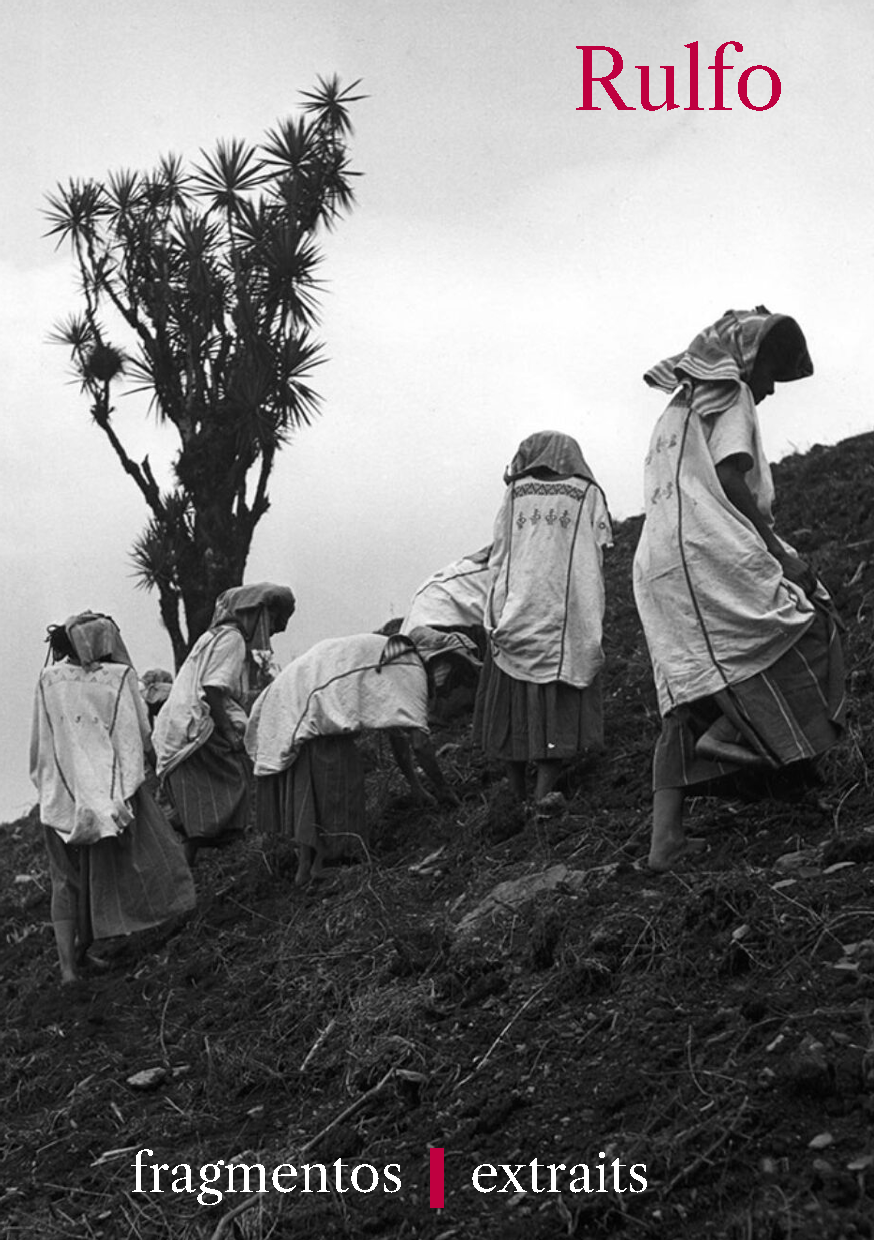
\includepdf{couverture/couverture.pdf}
\end{titlepage}

%\myemptypage
\thispagestyle{empty}
\vspace*{\fill}
\begin{center}
	\begin{minipage}{11em}
		Couverture: Juan Rulfo, \textit{Campesinas de Oaxaca}
	\end{minipage}
\end{center}
%\vspace*{\fill}
\addtocounter{page}{-1}
\newpage

\myemptypage

\importbilingualpages{parties/esquesomosmuypobres}%
{Es que somos muy pobres}{texte_es.tex}%
{C'est qu'on est très pauvres}{texte_fr.tex}

\importbilingualpages{parties/frag13}%
{Fragmento \esno 13}{texte_es.tex}%
{Fragment \frno 13}{texte_fr.tex}

\importbilingualpages{parties/frag16}%
{Fragmento \esno 16}{texte_es.tex}%
{Fragment \frno 16}{texte_fr.tex}

\end{document}
